\documentclass[10pt]{article}
\usepackage[polish]{babel}
\usepackage[utf8]{inputenc}
\usepackage[T1]{fontenc}
\usepackage{amsmath}
\usepackage{amsfonts}
\usepackage{amssymb}
\usepackage[version=4]{mhchem}
\usepackage{stmaryrd}
\usepackage{graphicx}
\usepackage[export]{adjustbox}
\graphicspath{ {./images/} }

\begin{document}
\begin{enumerate}
  \item Wykaż, że jeżeli pewna liczba naturalna jest sumą dwóch kwadratów liczb naturalnych, to również jej trzynastokrotność ma tę własność
  \item W trójkącie ABC: C' to spodek wysokości opuszczonej z wierzchołka C, B' spodek wysokości opuszczonej z wierzchołka B, zaś M to środek boku BC. Udowodnij, że symetralna odcinka \(B^{\prime} C^{\prime}\) przechodzi przez punkt M\\
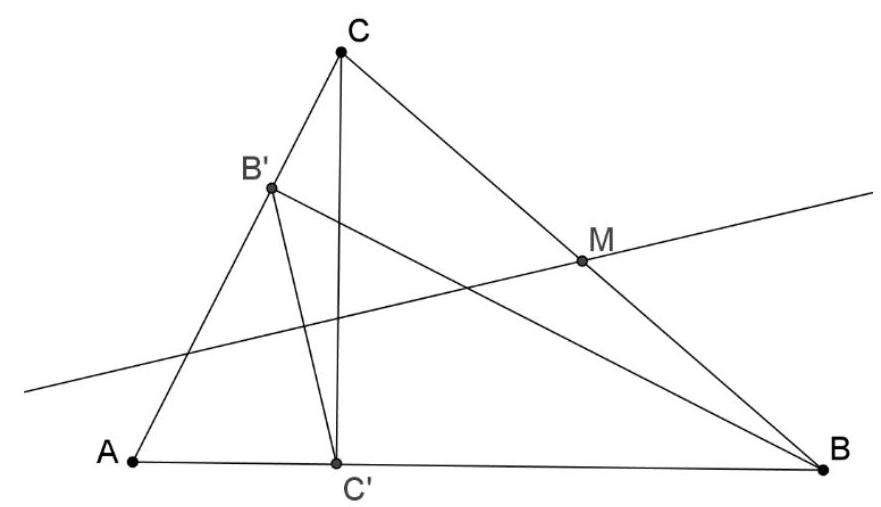
\includegraphics[max width=\textwidth, center]{2024_11_21_be053e1ed6379189d5d2g-1}
  \item Basia i Asia zbierały muchomory w lesie. Okazało się, że kropek na muchomorach Basi było 13 razy więcej niż na muchomorach Asi. Gdyby Basia oddała Asi swój muchomor z najmniejszą liczbą kropek, to wtedy u niej byłoby 8 razy więcej kropek niż u Asi. Oblicz, ile co najwyżej muchomorów mogła zebrać Basia?
\end{enumerate}

\end{document}